\documentclass[11pt,a4paper]{article}
\usepackage{gtu-el-yazisi}
\begin{document}
\notbilgi{İşaretler ve Sistemler}{Ders 5 -- Sürekli zamanlı Fourier serileri}{Isaret-ve-Sistemler-ders-5.pdf}
\renewcommand{\thempfootnote}{\alph{mpfootnote}} % kutu içi dipnotlar için (euler + \itshape uyumsuzluğu)

\section{Sürekli Zamanlı Fourier Serileri}
\sayfa{1}
(Continuous-Time Fourier Series)
\[ x(t) = x(t+T), \ \forall t \]
Periyodik bir işaret Fourier serisine açılabilir.

\subsection{Fourier Serisinin mevcut olma koşulları \normalfont(Dirichlet condition)}
\begin{enumerate}[label=\arabic*)]
  \item $x(t)$ işareti, bir periyot boyunca mutlak integrallenebilir olmalıdır.
  \[ \int_{0}^{T_0} |x(t)|\,dt < \infty \]
  Zayıf Dirichlet koşulu (weak Dirichlet condition)

  Bu koşul sağlanırsa Fourier serisi vardır, ancak seri her noktada yakınsamayabilir.
  \item $x(t)$ işareti, bir periyot boyunca
  \begin{itemize}[label=--]
    \item sonlu sayıda maksimum ve minimum değere sahip olmalıdır.
    \item sonlu sayıda süreksizliğe sahip olmalıdır ve bu süreksizlik noktalarında $x(t)$ işareti sonlu değer almalıdır.
  \end{itemize}
\end{enumerate}
Strong Dirichlet condition (1 ve 2)

Bu koşullar sağlanırsa Fourier serisi vardır.

(Bu şartların sağlanmadığı durumlarda da Fourier seri açılımı olabilir.)

\begin{itemize}[label=--]
  \item Genelleştirilmiş Fourier Serisi (Generalized FS)
  \item Trigonometrik Fourier Serisi (Trigonometric FS)
  \item Compact FS
  \item Üstel Fourier Serisi (Exponential FS)
\end{itemize}

\subsection{Ortogonal/ortonormal işaretler}
\sayfa{2}
$[t_1, t_2]$, \ $\psi_i(t)$, \ $-\infty < i < \infty$
\[ \int_{t_1}^{t_2} \psi_n(t)\,\psi_m^{*}(t)\,dt = \begin{cases} E_m, & m = n \\ 0, & m \neq n \end{cases} \qquad \text{ise } \psi_n(t) \text{ ve } \psi_m(t) \text{ işaretleri birbirine diktir (ortogonal).} \]
$E_m = 1$ ise $\psi_m(t)$ ve $\psi_n(t)$ ortonormal işaretlerdir.

\subsection{Genelleştirilmiş FS açılımı}
\[ x(t) = \sum_{k=-\infty}^{\infty} c_k\,\psi_k(t), \quad [t_1, t_2] \qquad \psi_k(t): \text{Temel fonksiyonlar (Basis functions)} \]
\[ c_k = \frac{1}{E_k}\int_{t_1}^{t_2} x(t)\,\psi_k^{*}(t)\,dt \]

\subsection{Üstel Fourier Serisi Açılımı \normalfont(Exponential FS Expansion)}
\[ x(t) = \sum_{k=-\infty}^{\infty} x_k\,e^{jk\omega_0 t}, \qquad t_1 \leq t \leq t_1 + T_0, \quad \omega_0 = 2\pi f_0 = \frac{2\pi}{T_0} \]
\[ x_k = \frac{1}{T_0}\int_{T_0} x(t)\,e^{-jk\omega_0 t}\,dt \]
$\Rightarrow$ $e^{jk\omega_0 t}$ : Temel fonksiyonlar
\[ \int_{0}^{T_0} e^{jk\omega_0 t}\cdot e^{-jn\omega_0 t}\,dt = \int_{0}^{T_0} e^{j(k-n)\omega_0 t}\,dt = \int_{0}^{T_0} \cos(k-n)\omega_0 t\,dt + j\int_{0}^{T_0} \sin(k-n)\omega_0 t\,dt = \begin{cases} T_0, & k = n \\ 0, & k \neq n \end{cases} \]
\[ \int_{T_0} x(t)\,e^{-jn\omega_0 t}\,dt = \sum_{k=-\infty}^{\infty} x_k \int_{T_0} e^{jk\omega_0 t}\cdot e^{-jn\omega_0 t}\,dt \underset{\substack{\uparrow\\ n=k}}{=} T_0\,x_k \longrightarrow x_k = \frac{1}{T_0}\int_{T_0} x(t)\,e^{-jk\omega_0 t}\,dt \]
$\Rightarrow$ $k = 0$
\[ x_0 = \frac{1}{T_0}\int_{T_0} x(t)\,dt \ : \ x(t) \text{ işaretinin bir periyodundaki ortalamasıdır.} \]

\subsection{Trigonometrik Fourier Serisi Açılımı}
\[ x(t) = a_0 + \sum_{k=1}^{\infty} a_k\cos k\omega_0 t + b_k\sin k\omega_0 t, \qquad t_1 \leq t \leq t_1 + T_0, \quad \omega_0 = \frac{2\pi}{T_0} \]
\begin{align*}
  a_k &= \frac{2}{T_0}\int_{T_0} x(t)\cos(k\omega_0 t)\,dt \\
  b_k &= \frac{2}{T_0}\int_{T_0} x(t)\sin(k\omega_0 t)\,dt \\
  a_0 &= \frac{1}{T_0}\int_{T_0} x(t)\,dt
\end{align*}

$\Rightarrow$ $\cos(k\omega_0 t)$ ve $\sin(k\omega_0 t)$ : Temel fonksiyonlar
\sayfa{3}
\begin{align*}
  & \int_{T_0} \cos(k\omega_0 t)\sin(n\omega_0 t)\,dt = 0 \\
  & \int_{T_0} \cos(k\omega_0 t)\cos(n\omega_0 t)\,dt = \begin{cases} T_0/2, & n = k \\ 0, & n \neq k \end{cases} \\
  & \int_{T_0} \sin(k\omega_0 t)\sin(n\omega_0 t)\,dt = \begin{cases} T_0/2, & n = k \\ 0, & n \neq k \end{cases}
\end{align*}
$\Rightarrow$ $x(t)$ işareti \textbf{tek} işaret ise $a_0 = a_n = 0$

\phantom{$\Rightarrow$ $x(t)$ işareti }\textbf{Çift} işaret ise $b_n = 0$

\begin{align*}
  \Rightarrow x(t) = \sum_{k=-\infty}^{\infty} x_k\,e^{jk\omega_0 t} &= x_0 + \sum_{k=1}^{\infty} x_k\,e^{jk\omega_0 t} + x_{-k}\,e^{-jk\omega_0 t} \\
  &= x_0 + \sum_{k=1}^{\infty} (x_k + x_{-k})\cos k\omega_0 t + j\,(x_k - x_{-k})\sin k\omega_0 t \\
  &= a_0 + \sum_{k=1}^{\infty} a_k\cos k\omega_0 t + j\,b_k\sin\omega_0 t \quad \longleftarrow \ \begin{aligned} a_0 &= x_0 \\ a_k &= x_k + x_{-k} \\ b_k &= x_k - x_{-k} \end{aligned}
\end{align*}

\subsection{Compact Fourier Series Expansion}
\[ a_k\cos k\omega_0 t + b_k\sin k\omega_0 t = c_k\cos(k\omega_0 t + \theta_k) \longleftarrow c_k = \sqrt{a_k^2 + b_k^2} \qquad \theta_k = -\arctan\left(\frac{b_k}{a_k}\right) \]
\[ x(t) = c_0 + \sum_{k=1}^{\infty} c_k\cos(k\omega_0 t + \theta_k), \qquad t_1 \leq t \leq t_1 + T_0 \]

\subsection{Fourier Spektrumu}
\[ \left.\begin{aligned} & c_k: \text{genlik spektrumu (amplitude spectrum)} \\ & \theta_k: \text{faz spektrumu (phase spectrum)} \end{aligned}\ \right\}\ \text{frequency spectra (frekans spektrumları)} \]

$\Rightarrow$ $x_0 = c_0 = a_0$
\[ x_k = \frac{1}{2}c_k\,e^{j\theta_k} = \frac{a_k - j b_k}{2} \qquad x_{-k} = \frac{1}{2}c_k\,e^{-j\theta_k} = \frac{a_k + j b_k}{2}, \quad k = 1, 2, \ldots, \infty \]

\begin{align*}
  \Rightarrow c_k\cos(k\omega_0 t + \theta_k) &= \frac{c_k}{2}\left[e^{j(k\omega_0 t + \theta_k)} + e^{-j(k\omega_0 t + \theta_k)}\right] \\
  &= \frac{c_k}{2}\,e^{j\theta_k}\,e^{jk\omega_0 t} + \frac{c_k}{2}\,e^{-j\theta_k}\cdot e^{-jk\omega_0 t} \\
  &= x_k\,e^{jk\omega_0 t} + x_{-k}\,e^{-jk\omega_0 t} \quad \longleftarrow \ \begin{aligned} x_k &= \frac{c_k}{2}\,e^{j\theta_k} \\ x_{-k} &= \frac{c_k}{2}\,e^{-j\theta_k} \end{aligned}
\end{align*}

$\Rightarrow$ Üstel Fourier spektrumu
\sayfa{4}
\begin{align*}
  & |x_k| = |x_{-k}| = \frac{1}{2}c_k \longrightarrow \text{genlik spektrumu çift simetriktir.} \\
  & \angle x_k = \theta_k, \quad \angle x_{-k} = -\theta_k \longrightarrow \text{faz spektrumu tek simetriktir.} \\
  & x_k = |x_k|\,e^{j\theta_k} \qquad x_{-k} = |x_{-k}|\,e^{-j\theta_k} = |x_k|\,e^{-j\theta_k}
\end{align*}

\begin{ornek}[(Ex)]
\begin{center}
\begin{tikzpicture}[xscale=2.6, yscale=0.9]
  \draw[->] (-1.9,0) -- (3.0,0) node[right] {$t$};
  \draw[->] (0,0) -- (0,1.6) node[right] {$x(t)$};
  \foreach \c in {-1,0,1,2} { \draw[thick] ({\c-0.25},0) -- ({\c-0.25},1) -- ({\c+0.25},1) -- ({\c+0.25},0); }
  \node at (-1.65,0.5) {$\cdots$};
  \node at (2.6,0.5) {$\cdots$};
  \node[above right] at (0,1) {\small $1$};
  \foreach \x/\l in {-1/{-T},-0.5/{-\frac{T}{2}},-0.25/{-\frac{T}{4}},0.25/{\frac{T}{4}},0.5/{\frac{T}{2}},1/{T},2/{2T}} { \draw (\x,0.07) -- (\x,-0.07); \node[below] at (\x,-0.05) {\small $\l$}; }
\end{tikzpicture}
\end{center}
\end{ornek}
\begin{cozum}
\textbf{a) Trigonometrik FS}
\[ x(t) = a_0 + \sum_{k=1}^{\infty} a_k\cos k\omega_0 t + b_k\sin k\omega_0 t, \qquad \omega_0 = \frac{2\pi}{T} = 2\pi f \]
\begin{align*}
  a_0 &= \frac{1}{T_0}\int_{T_0} x(t)\,dt = \frac{1}{T}\int_{-T/4}^{T/4} dt = \frac{1}{T}\left[\frac{T}{4} - \left(-\frac{T}{4}\right)\right] = \frac{1}{2} \\
  a_k &= \frac{2}{T_0}\int_{T_0} x(t)\cos k\omega_0 t\,dt = \frac{2}{T}\int_{-T/4}^{T/4} \cos k\omega_0 t = \frac{2}{T}\,\frac{\sin k\omega_0 t}{k\omega_0}\Bigg|_{-T/4}^{T/4} \underset{\substack{\uparrow\\ \omega_0 T\,=\,2\pi}}{=} \frac{1}{\pi k}\left[\sin k\omega_0\frac{T}{4} - \sin k\omega_0\frac{-T}{4}\right]
\end{align*}
\[ a_k = \frac{2}{\pi k}\sin\left(\frac{k\pi}{2}\right) = \begin{cases} 0, & k \text{ çift} \\[1mm] \dfrac{2}{\pi k}, & k = 1, 5, 9, \ldots \\[3mm] \dfrac{-2}{\pi k}, & k = 3, 7, 11, \ldots \end{cases} \]
$b_k = 0 \longleftarrow x(t) = x(-t)$ çift işaret olduğundan
\[ x(t) = \frac{1}{2} + \frac{2}{\pi}\left[\cos\omega_0 t - \frac{1}{3}\cos 3\omega_0 t + \frac{1}{5}\cos 5\omega_0 t - \frac{1}{7}\cos 7\omega_0 t + \cdots\right] \]

\textbf{b) Compact FS}
\begin{align*}
  & x(t) = c_0 + \sum_{k=1}^{\infty} c_k\cos(k\omega_0 t + \theta_k) \\
  & c_0 = a_0 = \frac{1}{2} \\
  & c_k = \sqrt{a_k^2 + b_k^2} = a_k \quad \text{\footnotemark} \\
  & -\cos x = \cos(x - \pi)
\end{align*}
\[ x(t) = \frac{1}{2} + \frac{2}{\pi}\left[\cos\omega_0 t + \frac{1}{3}\cos(3\omega_0 t - \pi) + \frac{1}{5}\cos 5\omega_0 t + \frac{1}{7}\cos(7\omega_0 t - \pi) + \cdots\right] \]
\[ c_k = \begin{cases} 0, & k \text{ çift} \\[1mm] \dfrac{2}{\pi k}, & k \text{ tek} \end{cases} \qquad\qquad \theta_k = \begin{cases} 0, & k = 1, 5, 9, \ldots \\ -\pi, & k = 3, 7, 11, \ldots \end{cases} \]
\end{cozum}
\footnotetext{Claude notu: $b_k = 0$ olduğundan $c_k = \sqrt{a_k^2} = |a_k|$ olmalı (aşağıda da $c_k = \frac{2}{\pi k}$, yani $|a_k|$ kullanılmış).}

\sayfa{5}
\noindent
\begin{minipage}[t]{0.48\linewidth}
\centering
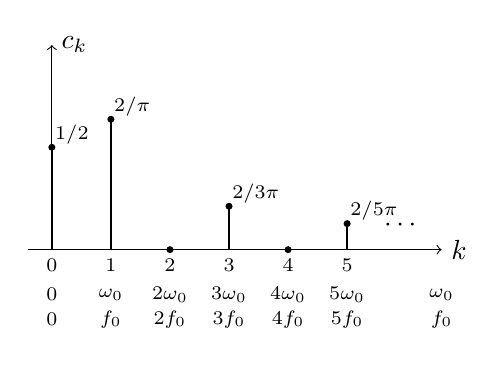
\begin{tikzpicture}[xscale=0.75, yscale=2.6]
  \draw[->] (-0.4,0) -- (6.6,0) node[right] {$k$};
  \draw[->] (0,0) -- (0,1) node[right] {$c_k$};
  \foreach \x/\y/\l in {0/0.5/{1/2},1/0.637/{2/\pi},3/0.212/{2/3\pi},5/0.127/{2/5\pi}} { \draw[thick] (\x,0) -- (\x,\y); \fill (\x,\y) circle (0.06 and 0.017); \node[above right, inner sep=1pt] at (\x,\y) {\scriptsize $\l$}; }
  \foreach \x in {2,4} { \fill (\x,0) circle (0.06 and 0.017); }
  \node at (5.9,0.12) {$\cdots$};
  \foreach \x in {0,...,5} { \node[below] at (\x,0) {\scriptsize $\x$}; }
  \node at (0,-0.22) {\scriptsize $0$}; \node at (1,-0.22) {\scriptsize $\omega_0$}; \node at (2,-0.22) {\scriptsize $2\omega_0$}; \node at (3,-0.22) {\scriptsize $3\omega_0$}; \node at (4,-0.22) {\scriptsize $4\omega_0$}; \node at (5,-0.22) {\scriptsize $5\omega_0$}; \node at (6.6,-0.22) {\scriptsize $\omega_0$};
  \node at (0,-0.34) {\scriptsize $0$}; \node at (1,-0.34) {\scriptsize $f_0$}; \node at (2,-0.34) {\scriptsize $2f_0$}; \node at (3,-0.34) {\scriptsize $3f_0$}; \node at (4,-0.34) {\scriptsize $4f_0$}; \node at (5,-0.34) {\scriptsize $5f_0$}; \node at (6.6,-0.34) {\scriptsize $f_0$};
\end{tikzpicture}

Genlik spektrumu
\end{minipage}\hfill
\begin{minipage}[t]{0.48\linewidth}
\centering
\begin{tikzpicture}[xscale=0.62, yscale=0.55]
  \draw[->] (-0.4,0) -- (8.2,0) node[right] {$k$};
  \draw[->] (0,-3.9) -- (0,1.6) node[right] {$\theta_k$};
  \foreach \x in {0,1,2,4,5,6} { \fill (\x,0) circle (2pt); \node[above] at (\x,0) {\scriptsize $\x$}; }
  \foreach \x in {3,7} { \draw[thick] (\x,0) -- (\x,-3.14); \fill (\x,-3.14) circle (2pt); \node[above] at (\x,0) {\scriptsize $\x$}; }
  \draw[dashed, kursunkalem] (0,-3.14) -- (7,-3.14);
  \node[left] at (0,-3.14) {\scriptsize $-\pi$};
  \node at (0.2,-4.5) {\scriptsize $0$}; \node at (1,-4.5) {\scriptsize $\omega_0$}; \node at (2,-4.5) {\scriptsize $2\omega_0$}; \node at (3,-4.5) {\scriptsize $3\omega_0$}; \node at (5,-4.5) {\scriptsize $\cdots$}; \node at (7,-4.5) {\scriptsize $7\omega_0\cdots$}; \node at (8.4,-4.5) {\scriptsize $\omega_0$};
  \node at (0.2,-5.3) {\scriptsize $0$}; \node at (1.4,-5.3) {\scriptsize $f_0\cdots$}; \node at (3,-5.3) {\scriptsize $3f_0$}; \node at (5,-5.3) {\scriptsize $\cdots$}; \node at (7,-5.3) {\scriptsize $7f_0\cdots$}; \node at (8.4,-5.3) {\scriptsize $f_0$};
\end{tikzpicture}

Faz spektrumu
\end{minipage}

\begin{cozum}
\textbf{c) Üstel FS}
\begin{align*}
  x(t) &= \sum_{k=-\infty}^{\infty} x_k\,e^{jk\omega_0 t} \\
  x_k &= \frac{1}{T_0}\int_{T_0} x(t)\,e^{-jk\omega_0 t}\,dt = \frac{1}{T}\int_{-T/4}^{T/4} e^{-jk\omega_0 t}\,dt = \frac{1}{T}\,\frac{e^{-jk\omega_0 t}}{-jk\omega_0} = \frac{-1}{jk\,2\pi}\left[e^{-jk\omega_0\frac{T}{4}} - e^{-jk\omega_0\frac{-T}{4}}\right] \\
  x_k &= \frac{1}{\pi k}\left[\frac{e^{jk\pi/2} - e^{-jk\pi/2}}{2j}\right] = \frac{1}{\pi k}\sin\left(\frac{k\pi}{2}\right)
\end{align*}
\[ x_0 = \frac{1}{2} \qquad x_1 = x_{-1} = \frac{1}{\pi} \qquad x_3 = x_{-3} = \frac{-1}{3\pi} \qquad x_5 = x_{-5} = \frac{1}{5\pi} \quad \cdots \]
\begin{center}
\begin{tikzpicture}[xscale=1.25, yscale=4.2]
  \draw[->] (-5.6,0) -- (5.8,0) node[right] {$k$};
  \foreach \x/\y in {0/0.5,1/0.318,-1/0.318,3/-0.106,-3/-0.106,5/0.064,-5/0.064} { \draw[thick] (\x,0) -- (\x,\y); \fill (\x,\y) circle (0.05 and 0.012); }
  \foreach \x in {-4,-2,2,4} { \fill (\x,0) circle (0.05 and 0.012); }
  \node[above] at (0,0.5) {\scriptsize $x_0 = \frac{1}{2}$};
  \node[above] at (1,0.318) {\scriptsize $1/\pi$}; \node[above] at (-1,0.318) {\scriptsize $1/\pi$};
  \node[above] at (5,0.064) {\scriptsize $1/5\pi$}; \node[above] at (-5,0.064) {\scriptsize $1/5\pi$};
  \node[right] at (3,-0.106) {\scriptsize $-1/3\pi$}; \node[right] at (-3,-0.106) {\scriptsize $-1/3\pi$};
  \node at (5.5,0.04) {$\cdots$};
  \foreach \x in {-5,-4,-2,-1,0,1,2,4} { \node[below] at (\x,0) {\scriptsize $\x$}; }
  \node[above] at (3,0) {\scriptsize $3$}; \node[above] at (-3,0) {\scriptsize $-3$};
  \node at (-1,-0.14) {\scriptsize $-\omega_0$}; \node at (0,-0.14) {\scriptsize $0$}; \node at (1,-0.14) {\scriptsize $\omega_0$}; \node at (2,-0.14) {\scriptsize $2\omega_0$}; \node at (3.2,-0.14) {\scriptsize $3\omega_0\ \cdots$}; \node at (5.6,-0.14) {\scriptsize $\omega_0$};
  \node at (0,-0.21) {\scriptsize $0$}; \node at (1,-0.21) {\scriptsize $f_0$}; \node at (2,-0.21) {\scriptsize $2f_0$}; \node at (3.2,-0.21) {\scriptsize $3f_0\ \cdots$}; \node at (5.6,-0.21) {\scriptsize $f_0$};
\end{tikzpicture}
\end{center}

\noindent
\begin{minipage}[c]{0.45\linewidth}
Not: \ $\mathrm{sinc}(t) = \begin{cases} \dfrac{\sin(\pi t)}{\pi t}, & t \neq 0 \\[2mm] 1, & t = 0 \end{cases}$
\end{minipage}\hfill
\begin{minipage}[c]{0.52\linewidth}
\centering
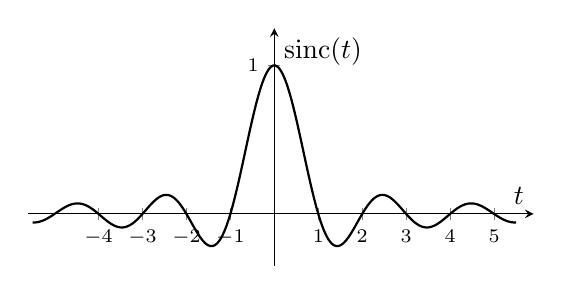
\begin{tikzpicture}
  \begin{axis}[width=8cm, height=4.6cm, axis lines=middle, xmin=-5.6, xmax=5.9, ymin=-0.35, ymax=1.25,
      xlabel={$t$}, ylabel={$\mathrm{sinc}(t)$}, xtick={-4,-3,-2,-1,1,2,3,4,5}, ytick={1},
      tick label style={font=\scriptsize}]
    \addplot[domain=-5.5:5.5, samples=200, smooth, thick] {sin(180*x)/(pi*x)};
  \end{axis}
\end{tikzpicture}

$t = k \in \mathbb{Z} - \{0\} \Rightarrow \mathrm{sinc}(t) = 0$
\end{minipage}

\[ \Rightarrow x_k = \frac{1}{\pi k}\sin\left(\frac{\pi k}{2}\right) = \frac{1}{2}\,\mathrm{sinc}(k/2) \]
\end{cozum}

$\Rightarrow$ Periyodik dikdörtgen dalga işaretinin üstel Fourier spektrumunun çizimi
\sayfa{6}
\begin{center}
\begin{tikzpicture}[xscale=3.2, yscale=0.9]
  \draw[->] (-1.7,0) -- (1.9,0) node[right] {$t$};
  \draw[->] (0,0) -- (0,1.6) node[right] {$x(t)$};
  \foreach \c in {-1,0,1} { \draw[thick] ({\c-0.3},0) -- ({\c-0.3},1) -- ({\c+0.3},1) -- ({\c+0.3},0); }
  \node at (-1.5,0.6) {$\cdots$}; \node at (1.55,0.6) {$\cdots$};
  \node[above right] at (0,1) {\small $A$};
  \foreach \x/\l in {-1/{-T_0},-0.5/{-\frac{T_0}{2}},-0.3/{-\frac{\tau}{2}},0.3/{\frac{\tau}{2}},0.5/{\frac{T_0}{2}},1/{T_0}} { \draw (\x,0.07) -- (\x,-0.07); \node[below] at (\x,-0.05) {\small $\l$}; }
\end{tikzpicture}
\end{center}
\[ x(t) = \sum_{k=-\infty}^{\infty} x_k\,e^{jk\omega_0 t} \]
\[ x_k = \frac{1}{T_0}\int_{T_0} x(t)\,e^{-jk\omega_0 t}\,dt = \frac{2A}{k\omega_0 T_0}\sin\left(k\omega_0\frac{\tau}{2}\right) \underset{\substack{\uparrow\\ \omega_0 T_0\,=\,2\pi\\ \omega_0\,=\,2\pi f_0}}{=} \frac{A}{\pi k}\sin(k\pi f_0\tau) \underset{\substack{\uparrow\\ f_0\tau\\ \text{çarp}\\ \text{böl}}}{=} A f_0\tau\,\frac{\sin(\pi k f_0\tau)}{\pi k f_0\tau} \]
\[ x_k = A f_0\tau\,\mathrm{sinc}(k f_0\tau) \]

$3f_0 < 1/\tau < 4f_0$ olsun.

\begin{center}
\begin{tikzpicture}[xscale=0.75, yscale=2.4]
  \draw[->] (-4.6,0) -- (8.4,0) node[right] {$f$};
  \draw[->] (0,0) -- (0,1.3) node[right] {$|x_k|$};
  \draw[dashed, kursunkalem, domain=-4.2:-0.05, samples=60] plot (\x, {abs(sin(180*\x/3.4)/(pi*\x/3.4))});
  \draw[dashed, kursunkalem, domain=0.05:8, samples=100] plot (\x, {abs(sin(180*\x/3.4)/(pi*\x/3.4))});
  \foreach \x/\y in {-3/0.130,-2/0.521,-1/0.864,0/1,1/0.864,2/0.521,3/0.130,4/0.143,5/0.216,6/0.122,7/0.028} { \draw[thick] (\x,0) -- (\x,\y); \fill (\x,\y) circle (0.065 and 0.02); }
  \node at (-4.3,0.12) {\scriptsize $\cdots$}; \node at (8.1,0.12) {\scriptsize $\cdots$};
  \foreach \x/\l in {-2/{-2f_0},-1/{-f_0},0/{0},1/{f_0},2/{2f_0},3/{3f_0}} { \node[below] at (\x,0) {\scriptsize $\l$}; }
  \foreach \x/\l in {4/{4f_0},5/{5f_0},6/{6f_0}} { \node[above] at (\x,0.22) {\scriptsize $\l$}; }
  \draw[->] (-3.4,-0.02) -- (-3.4,-0.2) node[below] {\scriptsize $-\frac{1}{\tau}$};
  \draw[->] (3.4,-0.02) -- (3.4,-0.2) node[below] {\scriptsize $\frac{1}{\tau}$};
  \draw[->] (6.8,-0.02) -- (6.8,-0.2) node[below] {\scriptsize $\frac{2}{\tau}$};
\end{tikzpicture}

Genlik spektrumu (Çift fonksiyon)
\end{center}
\begin{center}
\begin{tikzpicture}[xscale=0.62, yscale=0.42]
  \draw[->] (-7.8,0) -- (8.4,0) node[right] {$f$};
  \draw[->] (0,-4.2) -- (0,4.4) node[right] {$\theta_k$};
  \draw (-0.15,3.14) -- (0.15,3.14) node[right] {\scriptsize $\pi$};
  \draw (-0.15,-3.14) -- (0.15,-3.14) node[left=2pt] {\scriptsize $-\pi$};
  \foreach \x in {-6,-5,-4} { \draw[thick] (\x,0) -- (\x,3.14); \fill (\x,3.14) circle (2.2pt); }
  \foreach \x in {4,5,6} { \draw[thick] (\x,0) -- (\x,-3.14); \fill (\x,-3.14) circle (2.2pt); }
  \foreach \x in {-7,-3,-2,-1,1,2,3,7} { \fill (\x,0) circle (2.2pt); }
  \foreach \x/\l in {-3/{-3f_0},-2/{-2f_0},-1/{-f_0},1/{f_0},2/{2f_0},3/{3f_0},4/{4f_0},5/{5f_0},6/{6f_0},7/{7f_0}} { \node[above] at (\x,0.15) {\scriptsize $\l$}; }
\end{tikzpicture}

Faz spektrumu (Tek fonksiyon)
\end{center}

\begin{ornek}[(Ex)]
\noindent
\begin{minipage}[c]{0.42\linewidth}
\centering
\begin{tikzpicture}[xscale=0.8, yscale=0.9]
  \draw[->] (-3,0) -- (3.2,0) node[right] {$t$};
  \draw[->] (0,0) -- (0,1.6) node[right] {$x(t)$};
  \foreach \x in {-2,-1,0,1,2} { \draw[->, thick] (\x,0) -- (\x,1); }
  \draw[dashed, kursunkalem] (-2.6,1) -- (2.6,1);
  \node at (-2.6,0.5) {$\cdots$}; \node at (2.6,0.5) {$\cdots$};
  \foreach \x/\l in {-1/{-T},0/{0},1/{T},2/{2T}} { \node[below] at (\x,0) {\small $\l$}; }
\end{tikzpicture}
\end{minipage}\hfill
\begin{minipage}[c]{0.55\linewidth}
$x(t) = \displaystyle\sum_{k=-\infty}^{\infty} \delta(t - kT)$ \ dürtü katarı (impulse train)

\medskip
Üstel FS açılımını bulunuz.
\end{minipage}
\end{ornek}
\begin{cozum}
\begin{align*}
  x(t) &= \sum_{k=-\infty}^{\infty} x_k\,e^{jk\omega_0 t} \\
  x_k &= \frac{1}{T_0}\int_{T_0} x(t)\,e^{-jk\omega_0 t}\,dt = \frac{1}{T}\underbrace{\int_{-T/2}^{T/2} \delta(t)\,e^{-jk\omega_0 t}\,dt}_{=\,1} = \frac{1}{T}
\end{align*}
\begin{center}
\begin{tikzpicture}[xscale=1.3, yscale=0.9]
  \draw[->] (-2.8,0) -- (3.4,0) node[right] {$\omega$};
  \draw[->] (0,0) -- (0,1.7) node[right] {$x_k$};
  \foreach \x in {-2,-1,0,1,2} { \draw[->, thick] (\x,0) -- (\x,1); }
  \draw[dashed, kursunkalem] (-2.6,1) -- (0,1);
  \node[above right] at (0,1) {\small $1/T$};
  \node at (2.7,0.5) {$\cdots$};
  \foreach \x/\l in {-2/{-2\omega_0},-1/{-\omega_0},0/{0},1/{\omega_0},2/{2\omega_0}} { \node[below] at (\x,0) {\small $\l$}; }
\end{tikzpicture}
\end{center}
\end{cozum}

\begin{ornek}[(Ex)]
\sayfa{7}
$x(t) = 1 + \sin\omega_0 t + 2\cos\omega_0 t + \cos\left(2\omega_0 t + \pi/4\right)$
\end{ornek}
\begin{cozum}
\begin{align*}
  x(t) &= 1 + \frac{1}{2j}\left[e^{j\omega_0 t} - e^{-j\omega_0 t}\right] + e^{j\omega_0 t} + e^{-j\omega_0 t} + \frac{1}{2}\left[e^{j(2\omega_0 t + \pi/4)} + e^{-j(2\omega_0 t + \pi/4)}\right] \\
  &= 1 + \left(1 + \frac{1}{2j}\right)e^{j\omega_0 t} + \left(1 - \frac{1}{2j}\right)e^{-j\omega_0 t} + \frac{1}{2}e^{j\pi/4}e^{j2\omega_0 t} + \frac{1}{2}e^{-j\pi/4}e^{-j2\omega_0 t}
\end{align*}
\begin{align*}
  & x_0 = 1 \qquad && x_1 = 1 + \frac{1}{2j} = 1 - \frac{1}{2}j \qquad && x_2 = \frac{1}{2}e^{j\pi/4} = \frac{\sqrt{2}}{4}(1+j) \qquad && x_k = 0, \ |k| > 2 \\
  & && x_{-1} = 1 - \frac{1}{2j} = 1 + \frac{1}{2}j && x_{-2} = \frac{1}{2}e^{-j\pi/4} = \frac{\sqrt{2}}{4}(1-j)
\end{align*}

\noindent
\begin{minipage}[t]{0.5\linewidth}
\centering
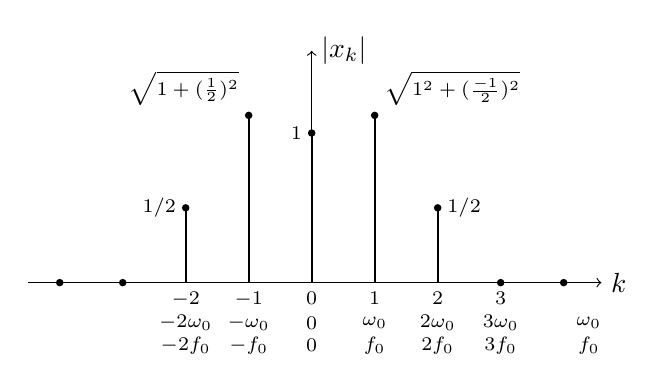
\begin{tikzpicture}[xscale=0.8, yscale=1.9]
  \draw[->] (-4.5,0) -- (4.6,0) node[right] {$k$};
  \draw[->] (0,0) -- (0,1.55) node[right] {$|x_k|$};
  \foreach \x/\y in {-2/0.5,-1/1.118,0/1,1/1.118,2/0.5} { \draw[thick] (\x,0) -- (\x,\y); \fill (\x,\y) circle (0.06 and 0.025); }
  \foreach \x in {-4,-3,3,4} { \fill (\x,0) circle (0.06 and 0.025); }
  \node[left] at (-2,0.5) {\scriptsize $1/2$}; \node[right] at (2,0.5) {\scriptsize $1/2$};
  \node[left] at (0,1) {\scriptsize $1$};
  \node[above left] at (-1,1.118) {\scriptsize $\sqrt{1 + (\frac{1}{2})^2}$};
  \node[above right] at (1,1.118) {\scriptsize $\sqrt{1^2 + (\frac{-1}{2})^2}$};
  \foreach \x in {-2,-1,0,1,2,3} { \node[below] at (\x,0) {\scriptsize $\x$}; }
  \node at (-2,-0.27) {\scriptsize $-2\omega_0$}; \node at (-1,-0.27) {\scriptsize $-\omega_0$}; \node at (0,-0.27) {\scriptsize $0$}; \node at (1,-0.27) {\scriptsize $\omega_0$}; \node at (2,-0.27) {\scriptsize $2\omega_0$}; \node at (3,-0.27) {\scriptsize $3\omega_0$}; \node at (4.4,-0.27) {\scriptsize $\omega_0$};
  \node at (-2,-0.42) {\scriptsize $-2f_0$}; \node at (-1,-0.42) {\scriptsize $-f_0$}; \node at (0,-0.42) {\scriptsize $0$}; \node at (1,-0.42) {\scriptsize $f_0$}; \node at (2,-0.42) {\scriptsize $2f_0$}; \node at (3,-0.42) {\scriptsize $3f_0$}; \node at (4.4,-0.42) {\scriptsize $f_0$};
\end{tikzpicture}

Genlik spektrumu
\end{minipage}\hfill
\begin{minipage}[t]{0.48\linewidth}
\centering
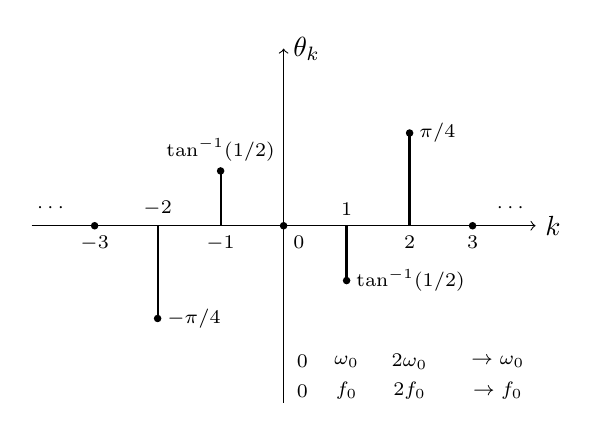
\begin{tikzpicture}[xscale=0.8, yscale=1.5]
  \draw[->] (-4,0) -- (4,0) node[right] {$k$};
  \draw[->] (0,-1.5) -- (0,1.5) node[right] {$\theta_k$};
  \foreach \x/\y in {-2/-0.785,-1/0.464,1/-0.464,2/0.785} { \draw[thick] (\x,0) -- (\x,\y); \fill (\x,\y) circle (0.06 and 0.032); }
  \foreach \x in {-3,0,3} { \fill (\x,0) circle (0.06 and 0.032); }
  \node at (-3.7,0.15) {\scriptsize $\cdots$}; \node at (3.6,0.15) {\scriptsize $\cdots$};
  \node[above] at (-1,0.464) {\scriptsize $\tan^{-1}(1/2)$};
  \node[right] at (1,-0.464) {\scriptsize $\tan^{-1}(1/2)$};
  \node[right] at (2,0.785) {\scriptsize $\pi/4$};
  \node[right] at (-2,-0.785) {\scriptsize $-\pi/4$};
  \node[above] at (-2,0) {\scriptsize $-2$}; \node[below] at (-3,0) {\scriptsize $-3$}; \node[below] at (-1,0) {\scriptsize $-1$}; \node[below right] at (0,0) {\scriptsize $0$}; \node[above] at (1,0) {\scriptsize $1$}; \node[below] at (2,0) {\scriptsize $2$}; \node[below] at (3,0) {\scriptsize $3$};
  \node at (0.3,-1.15) {\scriptsize $0$}; \node at (1,-1.15) {\scriptsize $\omega_0$}; \node at (2,-1.15) {\scriptsize $2\omega_0$}; \node at (3.4,-1.15) {\scriptsize $\rightarrow \omega_0$};
  \node at (0.3,-1.4) {\scriptsize $0$}; \node at (1,-1.4) {\scriptsize $f_0$}; \node at (2,-1.4) {\scriptsize $2f_0$}; \node at (3.4,-1.4) {\scriptsize $\rightarrow f_0$};
\end{tikzpicture}

Faz spektrumu
\end{minipage}
\end{cozum}

\end{document}
